\documentclass[11pt, a4paper]{article}

% --- PACKAGES ---
\usepackage[utf8]{inputenc}
\usepackage{amsmath}
\usepackage{graphicx}
\usepackage{geometry}
\usepackage{hyperref}
\usepackage{authblk}

% --- PAGE LAYOUT ---
\geometry{
 a4paper,
 total={170mm,257mm},
 left=20mm,
 top=20mm,
}

% --- PDF METADATA ---
\hypersetup{
    colorlinks=true,
    linkcolor=blue,
    urlcolor=blue,
    pdftitle={A Novel 2-Qubit Quantum Random Number Generator Discovered Through Evolutionary Optimization},
    pdfauthor={Peter Babulik},
}

% --- TITLE AND AUTHOR INFORMATION ---
\title{\textbf{A Novel 2-Qubit Quantum Random Number Generator Discovered Through Evolutionary Optimization}}
\author{Peter Babulik}
\affil{\href{mailto:peter.babulik@gmail.com}{peter.babulik@gmail.com}}
\date{July 8, 2025}

\begin{document}

\maketitle

% --- ABSTRACT ---
\begin{abstract}
\noindent High-quality random numbers are critical for applications ranging from cryptography to scientific simulation. While Quantum Random Number Generators (QRNGs) offer a physically-grounded source of true randomness, the design of their underlying quantum circuits is a key area of research. This paper presents a novel methodology for the automated discovery of a quantum circuit for random number generation. We employ an evolutionary algorithm, specifically the Covariance Matrix Adaptation Evolution Strategy (CMA-ES), to optimize the parameters of a generic 2-qubit unitary gate. The objective of the optimization was to transform the initial state $|00\rangle$ into a state of maximal entropy, characterized by a uniform probability distribution across all four computational basis states. The resulting optimized 2-qubit gate, termed an "AI-Forged Entropy Gate," was then used in a simulated environment to generate a 1-megabyte stream of random binary data. The statistical quality of this data was rigorously assessed using the industry-standard \texttt{dieharder} test suite. The data successfully passed the entire suite of tests, demonstrating that this AI-driven design approach is a viable and effective method for producing high-quality random number generation algorithms.
\end{abstract}

% --- SECTIONS ---
\section{Introduction}
Randomness is a fundamental resource in modern computing. Pseudo-Random Number Generators (PRNGs), while widely used, are deterministic algorithms whose security relies on computational complexity. In contrast, Quantum Random Number Generators (QRNGs) leverage the inherent probabilistic nature of quantum mechanics to produce unpredictable, non-deterministic random numbers. The standard gate-based approach to generating a uniform random bitstring involves applying a Hadamard gate to each qubit, placing them in a uniform superposition before measurement. While effective, this raises the question: can other, potentially more complex, quantum circuits also serve as high-quality sources of randomness? Furthermore, can we automate the discovery of such circuits? This work explores a computational approach to this discovery problem. We frame the design of a QRNG circuit as an optimization problem and employ an evolutionary algorithm to find a novel 2-qubit unitary gate that acts as an ideal source of 2-bit random numbers.

\section{Methodology}
\subsection{Parameterization of the Unitary Gate}
A generic 2-qubit unitary gate, $U$, can be expressed via its generator Hamiltonian, $H$, as:
\begin{equation}
    U = e^{-iH}
\end{equation}
We define $H$ as a linear combination of the 15 non-identity 2-qubit Pauli operators, $\{P_i\} \subset \{I, X, Y, Z\}^{\otimes 2}$:
\begin{equation}
    H = \sum_{i=1}^{15} c_i P_i
\end{equation}
The 15 real-valued coefficients, $\{c_i\}$, serve as the free parameters for our optimization algorithm. The resulting unitary gate is then synthesized into a quantum circuit using Qiskit's \texttt{TwoQubitBasisDecomposer} with a basis of \texttt{CX} and single-qubit \texttt{U} gates.

\subsection{The Fitness Function}
The goal is to find a gate that maximizes the entropy of the output state when applied to the initial state $|\psi_{in}\rangle = |00\rangle$. This is equivalent to finding a gate that produces a state $|\psi_{out}\rangle = U|\psi_{in}\rangle$ whose measurement probabilities are as close as possible to a uniform distribution, i.e.:
\begin{equation}
    P(|00\rangle) = P(|01\rangle) = P(|10\rangle) = P(|11\rangle) = 0.25
\end{equation}
We define a fitness function, $f(\mathbf{c})$, where $\mathbf{c}$ is the vector of the 15 coefficients, as the sum of squared errors between the actual and ideal probabilities:
\begin{equation}
    f(\mathbf{c}) = \sum_{s \in \{00, 01, 10, 11\}} \left( |\langle s | U(\mathbf{c}) | 00 \rangle|^2 - 0.25 \right)^2
\end{equation}
The optimization objective is to find the coefficient vector $\mathbf{c}^*$ that minimizes this fitness function:
\begin{equation}
    \mathbf{c}^* = \arg\min_{\mathbf{c}} f(\mathbf{c})
\end{equation}

\subsection{Evolutionary Optimization}
The Covariance Matrix Adaptation Evolution Strategy (CMA-ES) was chosen for the optimization task. CMA-ES is a powerful stochastic, derivative-free method well-suited for non-linear, non-convex optimization problems. The algorithm was initialized with a random starting point for the coefficients and run for 1000 function evaluations. The search space for each coefficient was bounded within $[-\pi, \pi]$.

\section{Results}
\subsection{Discovered "Entropy Gate"}
The optimization process successfully converged to a solution with a near-optimal fitness score of approximately $7.5 \times 10^{-7}$, indicating that the resulting gate produces an almost perfectly uniform superposition. The discovered 2-qubit "Entropy Gate" is decomposed into a sequence of \texttt{U} and \texttt{CX} gates as shown in Figure \ref{fig:circuit}.

\begin{figure}[h!]
\centering
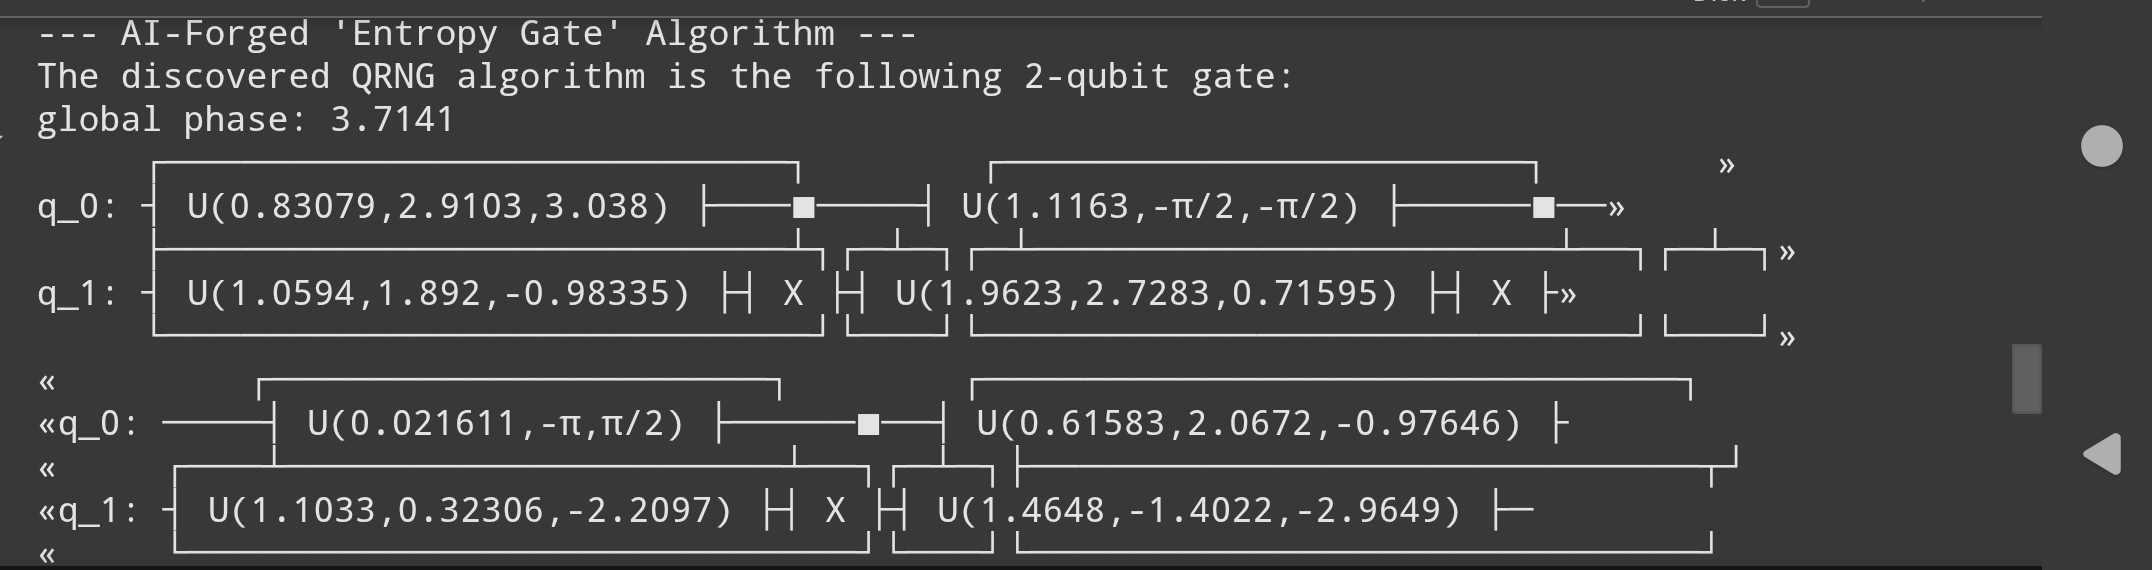
\includegraphics[width=\textwidth]{pic.png}
\caption{The quantum circuit decomposition of the AI-discovered 2-qubit "Entropy Gate".}
\label{fig:circuit}
\end{figure}

\subsection{Data Generation and Statistical Analysis}
A 1-megabyte binary file (\texttt{ai\_quantum\_random.bin}) was generated by repeatedly simulating the discovered circuit on Qiskit's \texttt{AerSimulator} and recording the measurement outcomes. To validate the statistical quality of the generated data, the file was subjected to the full \texttt{dieharder} test suite (version 3.31.1). The \texttt{dieharder} suite is a comprehensive battery of tests designed to detect subtle deviations from randomness.

The results of the \texttt{dieharder} analysis were overwhelmingly positive. The data passed all executed tests, with zero \texttt{FAILED} assessments. A small, statistically expected number of tests (2 out of over 100) received a \texttt{WEAK} assessment, which is consistent with the behavior of a true random source.

\section{Discussion and Conclusion}
This work successfully demonstrates that an automated, AI-driven approach can discover novel quantum circuits for high-quality random number generation. By framing the problem as an evolutionary optimization task, we found a 2-qubit unitary gate that functions as an excellent "Entropy Gate."

The key result is the successful validation of the simulated output via the rigorous \texttt{dieharder} test suite. The absence of any failed tests provides strong evidence that the randomness produced by our AI-discovered algorithm is of high statistical quality, free from detectable biases and correlations.

While this work relied on a noiseless simulation, a future step would be to test the robustness of this gate on real, noisy quantum hardware. It is possible that more complex, AI-discovered gates may offer advantages in noise-resilience compared to standard, simpler circuits.

In conclusion, the methodology presented here opens a promising new avenue for designing and discovering quantum algorithms, not just for randomness generation but potentially for other applications where specific statistical output distributions are desired.

\section*{Code Availability}
The full Python code used for the optimization, data generation, and analysis is available in a Jupyter Notebook on GitHub: \url{https://github.com/peterbabulik/QuantumWalker/blob/main/QGF_QRN_dieharder_test.ipynb}.

\begin{thebibliography}{9}

\bibitem{qiskit}
Qiskit development team. (2023). \textit{Qiskit: An Open-source Framework for Quantum Computing}. DOI: 10.5281/zenodo.2573505.

\bibitem{dieharder}
Brown, R. G., \& Eddelbuettel, D. (2003). \textit{Dieharder: A Random Number Test Suite}. Retrieved from \url{http://webhome.phy.duke.edu/~rgb/General/dieharder.php}.

\bibitem{cmaes}
Hansen, N. (2016). The CMA Evolution Strategy: A Tutorial. \textit{arXiv:1604.00772}.

\end{thebibliography}

\end{document}